\documentclass[11pt,letterpaper]{article}
\usepackage{naaclhlt2013}
\usepackage{times}
\usepackage{latexsym}
\usepackage{url}
\usepackage{graphicx}
\setlength\titlebox{6.5cm}

\title{Word Vector Representations for \\
Syntactically Disparate Event Descriptions}

\author{Travis Wolfe\\
	    Johns Hopkins University \\
	    {\tt travis@cs.jhu.edu}
}

\date{}

\begin{document}
\maketitle
\begin{abstract}
In this work we present an unsupervised method for
learning word vector representations that are conducive to
identifying coreferent mentions of events.
This is a hard problem because event mentions are weakly
tied to syntax and can be realized in may ways.
We discuss the justifications for a model that decomposes
coherence into syntactic and conceptual aspects and
provide a training procedure for it.
An evaluation framework is provided but without results due
to difficulty with numerical optimization.
\end{abstract}



\section{Introduction}
% 1 page
%%% GENERAL
Knowledge representations for events in natural language has been given many different treatments.
Much linguistic work does not concern itself with the problem of learning and
the representation on which they study linguistic regularities.
In NLP representations are often comprised of ad hoc feature and lists of
trigger words which are only available as long as there is an expert able to write them.
This data is often task specific and difficult to acquire.
Some annotated corpora have been created with frames or propositions labelled
in hopes that machine learning techniques might generalize this supervision to new data.
%Connectionists seek unification between the study of the neural representations
%of humans with practical tasks in NLP.
%This work most closely follows the connectionist track in trying to learn
%vector representations for words that allow us to make predictions about more
%abstract concepts in linguistics, like events and entities.
In this work, we propose an unsupervised model for learning event representations
based at the lexical level based on as little supervision and as much data
as possible.



%%% EVENTS
Our model of words decomposes words into the conceptual properties
of the predicates and arguments they evoke/describe and syntactic properties
of the words themselves.
As is generally true with unsupervised learning, you cannot learn
things that are not present in the data, so this goal of learning event
representations comes hand in hand with a hypothesis about the
distribution of event descriptions and their arguments.
The hypothesis is that there is regularity in the realization of predicates
and their arguments which is independent of syntax which can be observed
in local fragments of text.
% cite chomsky as decrying "linear order" in text, and then brush it off
Previous work in learning features for words has operated in the
paradigm of language modeling, and the features they learn are
interesting but constrained (c.f. related work).
The main drawback is that these representations do not allow generalization
across syntactic category.
This ability is paramount to modeling events because they can be described
in a wide variety of syntactic realizations.
Take Figure \ref{eventDesc} for example, which gives three descriptions of a wedding,
and note that
1) there is no clear syntactic correspondence between the descriptions
and 2) a good amount of information is captured near the event's trigger word in each case.

\begin{figure*}[ht]
\begin{tabular}{ | l | l | l | l | }
\hline
phrase & event trigger category & ARG0 category & ARGM category \\
\hline
Jane's joyous wedding & NN & NNP+POS & JJ \\
Jane was joyous when she got married & VB & NNP+PRP & JJ \\
Jane joyously gave her vows & VBD+PRP\$+VBZ & NNP & RB \\
\hline
\end{tabular}
\caption{three syntactically disparate descriptions of the same event}
\label{eventDesc}
\end{figure*}


The claim is not that arguments are always close, but
that they are biased towards being close\footnote{Grice's Maxim of Manner suggests
that the speaker should be brief. If the speaker is to be both brief and informative,
related concepts must appear close together.}
and when they are not close, the intervening words are not
systematically idiosyncratic to the event/predicate being described.

Thus we are beginning to describe a statistical theory of coherence
based on locality of predicate and argument trigger words.
What remains is to define mathematically how this coherence should be modeled.


\section{Model} %%%%%%%%%%%%%%%%%%%%%%%%%%%%%%%%%%%%%%%%%%%%%%%%%%%%%%%%%%%%%%%%%%%%%%%%
A primary goal of this work is to learn from unannotated text and
the simplest way to do this is via language modeling, i.e. inducing
a score or probability distribution over word sequences.
Previous work has shown that we can learn very fine grained information
by inducing features for a language model (c.f. related work).
While previous work has referred to this as language modeling,
this has the unwanted connotation that we are interested in the
numerical scores that come out of the language model for some NLP task.
Instead, we'll refer to our modeling as addressing {\em coherence},
and we'll discuss the factors that lead to coherence and how we might learn them. 
Later in section \ref{section:unlearnability}, we'll discuss ways in which our model of coherence
fails as a general explanation of coherence and how we might improve it.

Lets start with a simple model of coherence where we look at a small phrase of words
and decide if it is coherent. Since we don't know, or rather want to learn, how words
collocate and compose, we will impose very few restrictions on how the words might
interact in determining coherence. Lets use a single hidden layer neural network to
describe this process of determining coherence\footnote{Note that while describing
the properties of this network we will refer to this as a black box computational
unit that has capabilities to do things like compose and argmax vectors.
While it is outside of the scope of this work to explain the mechanisms by which this
occurs, single layer feed forward networks are universal function approximators \cite{Hornik:1989}
and can represent such computations with enough parameters and training data.
}.
The inputs to the network will be one
vector for every word in the phrase and the output will be a coherence score
(which we will refer to as $s(\cdot)$).
The hidden layer in the middle will store some notion of non-linear composition,
but we will not assume we know how to parse.

This network has the nice property that we can propagate a gradient all the
way from the output score back to the values in the word vectors.
We can then learn features for words by training the network to accomplish
a discriminative task that looks like comprehension.
Given a phrase $x$ and a corrupted (and hence incoherent) phrase $\tilde{x}$,
we want to train our model to recognize that the score of the uncorrupted phrase
is more coherent than the corrupted one: $s(x) \ge s(\tilde{x}) + 1$.
This training procedure, provided we can get coherent phrases and an automatic method of
corruption, means that we can train on as much unlabeled training data as we have.

The model just described closely resembles the model of \cite{rami}, and
can learn fine grained (seemingly) semantic similarities like ``Apple" is
similar to ``Dell" if you take similarity to mean cosine distance of the
vectors learned for ``Apple" and ``Dell".
The problem with this method is that you will learn that ``marry" and
``wedding" are very dissimilar. The reason for this is that they are from
different syntactic categories and you would never use one as a direct replacement
for the other.
If we want a more general notion of similarity, or in this case type-level event
coreference\footnote{type-level event coreference in the sense that instances may
not be coreferent, the phrase ``John married Mary" describes a different event from
``John and Mary's wedding", but holding the all of the arguments constant, coreference holds.},
then we need to relax the assumption of replaceability in a sequence of words with
a less syntax dependent notion of coherence.

One way to do this is to remove the order of the words in the sequence
(this is used in the CBOW method of \cite{DBLP:journals/corr/abs-1301-3781}),
but this throws the baby out with the bathwater. With no order you cannot
tell the difference between ``dog bites man" and ``man bites dog", and surely
you would learn a different conception of ``biting" if you thought people went
around doing it to dogs.
A more general way to state this is that syntax plays a role in semantic interpretation,
and we should not remove it entirely from our model of coherence.

Another way to remove the syntactic dependence is to consider that words that describe events that have
different syntactic category live in different places of the vector space
we are learning our representation in, but that there is some kind of mapping
between event descriptions. For example we might want to learn a transformation
on our vector space that takes the vector for ``marry" (in the verbal part
of the space) to a vector near ``wedding" (in the nominal part of the space).

% test on NOMLEX, performance is bad
We tested the plausibility of a model like this by trying to learn this type
of transformation on labelled pairs of nominal and verbal trigger words for events
like ``testament" and ``testify". This data was taken from NOMLEX \cite{nomlex},
which provides us with 3,135 noun-verb pairs.
We took the embeddings of \cite{rami} and tried to learn a linear map that minimized
the Euclidean distance between the vector representation for the noun $x_n$ and the
projected vector for the verb $x_v$:
\[
	\min_P \sum_{(n,v) \in \mbox{\texttt{NOMLEX}}}
		|| x_n - P x_v ||_2^2
\]

When we compared the error of this model (on training data), it
was not substantially lower than the variance from the mean of the nominal vectors,
$\sum ||x_n - E[x_n]||_2^2$, which indicates that this model has no hope
of relating this data in an accurate way. Nonlinear transforms were not attempted
due to the size of the data and the apparent difficulty of the mapping.


% shouldn't work anyway
On second inspection it doesn't seem like this method of projection would work for a few reasons.
First, since the word representations have not been preprocessed for polysemy, projection is much harder than
it would be if we assumed that we were projecting a centroid in some conceptual space\footnote{this
is assuming that the values in a word vector can represent either a point in space (a.k.a. a centroid)
or a distribution like one that you might get out of a feature vector in a log-linear model}.
If a word vector needs to store two meanings, e.g. ``testament" as in ``old" or as in what you do in court,
then the projection would need to preserve this polysemy, and in a way that represents the
syntactic category information, even if that notion might be null in some sense
(e.g. there is no verb that corresponds to the ``old testament" sense of ``testament" because it is not an event).
%also instance level info


We then return to our simpler model of coherence,
but try to force the vectors we learn for words to be less syntax dependent.
%One reason benefit of this model is that it can solve the polysemy problem by putting more
%infromation in the hidden layer via a weak form of composition\footnote{you
%might imagine weights leading into the hidden layer implementing a (soft)max
%over possible compositions}. 
We can do this by separately modeling the syntactic and conceptual aspects separately.
Lets define a word vector $v_i$ to be a composition of a vector representing its
syntactic properties $s_i$ and its non-syntactic properties $w_i$.
\[
	v_i = s_i \oplus w_i
\]
As before, we will build up a phrase vector $x$ by stacking the words in a phrase,
$x = [v_{i-k}, ..., v_i, ..., v_{i+k}]$, for some small context size $k$.
We want to come up with a way of learning $s_i$ in a way that will favor syntax and
be tied between various words (else we have something that is equivalent to the first model),
so we will represent $s_i$ as a row in a matrix $S_{t(i),\bullet}$,
where $t(i)$ is the part of speech tag of word $i$. In principle $t(i)$ could be more
fine grained than a part of speech tag, but it should be easily determined by surface
forms of the text so that it can be used on large unlabeled datasets.
We can also arrange all of the $w_i$ as rows in a matrix $W$.

With regard to how $\oplus$ should be implemented, we could use multiplication,
additions, or some other operator, but we favor vector stacking because it
implies that there are dimensions that account for syntactic versus semantic
coherence, a distinction which we intuitively believe to exist.
%First, vector stacking encodes the belief that syntax is a distinct property
%of words from their idiosyncratic meaning. % TODO support this
%Second, they are computationally more appealing because it 



\section{Learning} %%%%%%%%%%%%%%%%%%%%%%%%%%%%%%%%%%%%%%%%%%%%%%%%%%%%%%%%%%%%%%%%%%%%%%%%%%%%%%%
To train our model, we sought a large dataset that has many mentions of events,
so we opt for a corpus comprised of newswire text taken from the New York Times,
a part of the Annotated Gigaword dataset \cite{agiga}, ranging from 2000 to 2004.
This yields a dataset with 153,762 unique words and 456,746,432 phrases.
Given this corpus, we first give every word that appears at least 100
times an index and label all other words as \texttt{OOV}\footnote{we will learn
one vector for \texttt{OOV} even though there are many \texttt{OOV} words}.
Numbers are replaced by a unique token that only says how many digits are in
the token\footnote{e.g. ``120" $\rightarrow$ \texttt{3D} and ``1995" $\rightarrow$ \texttt{4D}}.
We then break text up in windows of size 5 ($k=2$) and shuffle all of the instances.

We need to choose the corruption model carefully because it affects the parameters we learn.
We follow \cite{rami} in that we only corrupt the middle word of the language model,
but we still have to decide whether to corrupt the word, its part of speech tag, or both.
In this work we do not consider perturbations of both because that leads to a very
diffuse gradient which updates both the $W$ and $S$ matrices rather than just one.
As a heuristic for when to perturb the word vs it's tag, we use
\[
	p(\mbox{perturb word}) = \frac
		{\sqrt{|W|} \times H(p_W)}
	{\sqrt{|W|} \times H(p_W) + \sqrt{|S|} \times H(p_S)}
\]
where $|W|$ is the number of parameters in the $W$ matrix, $H(\cdot)$ is
the entropy of a distribution, and $p_W$ and $p_S$ are the unigram distributions
of words and part of speech tags respectively\footnote{You could consider methods
that make a perturbation choice based on the phrase, but these methods are
substantially slower at training time or would require a lot of offline computation.
A careful implementation could do this efficiently, but that is not in the scope of this paper.
The method used in this paper only requires a few bits of entropy and no memory accesses.}.


The feedforward network was implemented in Theano \cite{theano},
a python library which provides automatic differentiation and support for GPU computing.
Training was run using a variant of batched stochastic gradient descent called AdaGrad \cite{adagrad}
\footnote{Batches of 500 examples worked best in our experiments}.
We set the dimension of both the syntactic and non-syntactic vectors to be 32
and the hidden layer to be 40
(on the small end of the spectrum with respect to previous work,
but the dimension tends to correlate with training time).









\section{Evaluation} %%%%%%%%%%%%%%%%%%%%%%%%%%%%%%%%%%%%%%%%%%%%%%%%%%%%%%%%%%%%%%%%%%%%%%%%%%%%%%%%
In order to evaluate our model, there are a few perspectives we can take.
The first question, is does our compositional model of coherence do any better
than the baseline model of one vector per word?

% d = read.csv('../vanilla-learn-curve.txt', header=F, sep=" ")
% plot(d)
From the learning curves, it appears that the baseline method outperforms
the two part model for the first 150 epochs. It is likely that this is due
to search error because the baseline is nested in the full model (functional subset).
It is not clear if more training time would alleviate this problem.
\begin{figure}[ht]
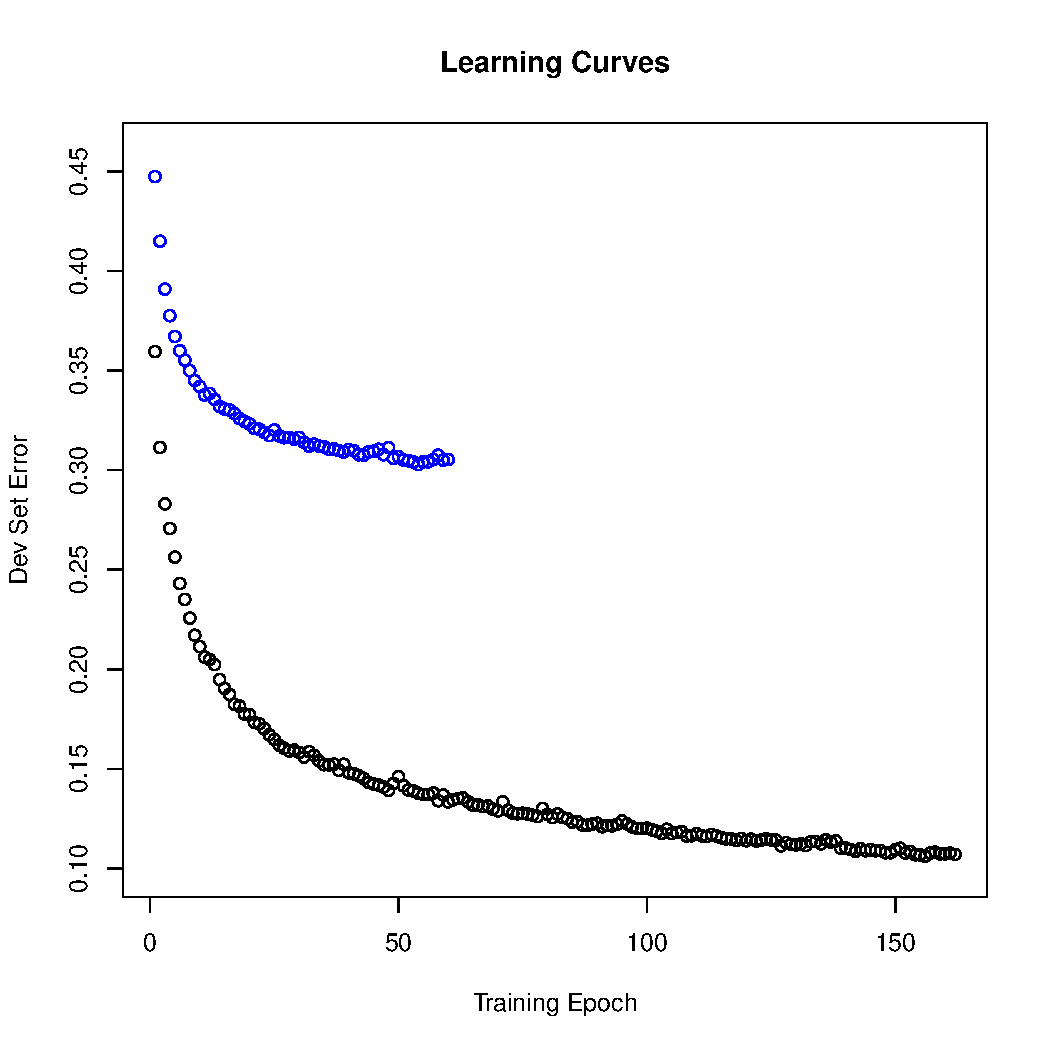
\includegraphics[width=\linewidth]{learningCurve.pdf}
\caption{Held out data learning curves for the baseline model (black) and the
decomposition model (blue). This is only the first few hours of training
due to a last minute bug fix.}
\end{figure}


%- pool all nomlex entries (which are words with POS)
%	lookup their C+S representation
%	for each pair (n,v):
%		sort all items by $dist(c(n), \cdot)$
%		compute rank of c(v) in this list
%	show a few of these nearest neighbor lists (include syntax dependent versions too)
%
%	compare this method to regular unsupervised + leave one out training of a non-linear projection of n->v
%
%- compare learning curves for C+S model vs plain W model

We also want to know about the nature of the syntax-stripped vectors we learn, in $W$.
In this work we have regarded the conceptual or semantic properties of a word simply as
the residual of what syntax doesn't explain. This notion is a bit unhelpful in light
of the fact that there are properties of words that we commonly refer to ``semantic" properties,
and we would like to know if we are learning a representation that speaks to these properties.
To explore one aspect of this, we consider a low-resource classification task where
the labels are semantic properties that do not seem to be related to the surface forms
of the words used to describe them, namely the event class of {\em State}, {\em Process},
and {\em Accomplishment}\footnote{data taken from \url{http://www.sfu.ca/person/dearmond/322/322.event.class.htm}}.
Given only 45 verbs across these classes, the leave-one-out accuracy of a classifier trained
on the representations of these words achieved 73\% accuracy, significantly greater than would
be achieved by guessing the most common class (36\%)\footnote{the vectors for this experiment
were taken from the baseline model}.
This indicates that whatever is being learned, it is correlated with at least one aspect of
what we consider to be relevant properties to the semantics of events.





\section{Shortcomings} %%%%%%%%%%%%%%%%%%%%%%%%%%%%%%%%%%%%%%%%%%%%%%%%%%%%%%%%%%%%%%%%%%%%%%%%%%%%%%
\label{section:unlearnability}
Though we have discussed our hypothesis of how predicate argument descriptions
appear in text, and how our model might learn from these patterns, it is worth
dwelling on the shortcomings of this model.

% no parsing
% locality
% no explicit argument structure
%	negative interaction between arguments is difficult if one is consistenly outside the window
The most obvious objection is that this model is very local in it's view of composition.
Long distance dependencies pose a problem in this model with respect to argument
interaction. If we assumed that arguments were independent conditioned on the predicate,
and that with some probability arguments appeared in the same phrase as their predicate,
then we might hope to learn the selectional preferences. However, if there are interactions
between the arguments, and we consistently see only some of the arguments in the phrase,
then the model has no way to tell if the argument is conditionally likely or not given
the limited information in the phrase.

Related to this objection is the objection that there is no parsing or modeling of
binary constituent unification.
The easiest and perhaps least satisfying response to this is that parsing and models
of larger spans of text are outside of our computational ability right now. To put this
in perspective, even with a model that was chosen for its computational efficiency like
this one, training high quality vectors can take three \cite{rami} to
eight \cite{DBLP:journals/corr/abs-1301-3781} {\em weeks} of CPU time.
This is not to detract from the value of these training routines, which should be weighed
against the main-years of effort required to come up with them.
But training on tree structure or wider windows will likely take advances in either
neural net training techniques or computational power.



% no instances
% no regular treatment of polysemy
Another problem with this model is that there is no explicit attempt to model
instances of data rather than types. That is, we learn representations for
words, but never reason explicitly about the meaning of a word in context aside
from the state of the hidden layer of the network. 
This means that ambiguity, be it introduced by polysemy or non-determinism in
composition, is reasoned about in an ad hoc and flat way.
Some work has addressed this problem \cite{multiplePrototypes1,multiplePrototypes2}.




% no formal semantics -> no worse than Hobbs, he provides no explanation of where predicates come from

% not grounded
Lastly, this model lives in an ungrounded paradigm of learning. Whatever it learns,
it learns from the New York Times, and can never observe any of the events described.
This means that it has no real sense of time or duration, but rather only represents
these concepts as far as they help explain the text it sees.
It is an open question of how much real world knowledge can be learn only from text
and whether this can be learned without a systematic prior or bias that is present only in humans.
The experiment concerning event class at least indicates that somethings that are
not obvious, like telicity, show up in a systematic enough way that the model can learn
something correlated with it.







%\section{Improvements}
%- train on dependency parses (not low resource)
%	- teaches you selectional preferences, but no better than the parser was!
%
%- train on consecutive verbs or subjects
%	- teaches you about discourse
%	- the event described before and after an event is likely to be relevant (e.g. scripts)
%
%- use bags of words related to an event with an intruder
%
%- adaptive corruption (more plausible interlopers)



\section{Related Work} %%%%%%%%%%%%%%%%%%%%%%%%%%%%%%%%%%%%%%%%%%%%%%%%%%%%%%%%%%%%%%%%%%%%%%%%%%%%%
Work in neural representations and language models has a long history
\cite{foundation1,foundation2,foundation3} inter alia,
and has recently regained a lot of attention.

% - scalar adjectives (deMarneffe)

% collobert and weston
\cite{DBLP:conf/icml/CollobertW08} built a multi-task NLP system based
on vector representation models which was trained to predict NER tags,
chunkings, and semantic role labelings. The SRL task is the most relevant
to this work, but their training procedure was fully supervised and
is differs greatly from this work.

% turian
\cite{turian} showed that features learned by
a few vector representation models improved the state of the art in NER tagging and chunking.


\cite{MikolovYZ13} analyzed the representations learned using
	a recurrent neural network language model described in \cite{DBLP:conf/interspeech/KombrinkMKB11}
which was initially created to aid in machine translation.
\cite{MikolovYZ13} however showed that the representations learned by the
language model were not only very good for that task, but also for the
task of analogy completion, which was one of the tasks in SemEval 2012 \cite{semeval2012}.

\cite{rami} presented a discriminatively trained feedforward neural network
which induces representations with similar properties to those learned using
a probabilistic language models, but with greatly accelerated training.
This model achieved state of the art part of speech tagging accuracy (or near it)
for many languages given only a very small labeled training set and the representations
learned on unlabeled data.
\cite{DBLP:journals/corr/abs-1301-3781} also focussed on efficient training and
proposed a similar model that sums rather than concatenates the input vectors,
and another that is just the reverse prediction task with the same network structure
(predict neighboring words from central word instead of central word from neighboring words).
The representations worked very well at analogies that represent specific lexical shifts
like pluralization (e.g. ``dog" : ``dogs" :: ``cat" : ``cats"), superlativization
(e.g. ``easy" : ``easiest" :: ``lucky" : ``luckiest"), and
capital cities (e.g. ``Athens" : ``Greece" :: ``Oslo" : ``Norway").
Their best model got 50.0\% accuracy on these tasks, but only one of the analogy types
reflected a change in syntactic category, which was between adjectives and adverbs.

%compare to Mikolov CBOW and other bag of words methods and say that
%what they get at is the same thing:
%removing order means that they are really working with conceptual coherence
%(and removing a lot of the syntactic requirements for coherence)
%BUT, not *all* information in the syntax/order is irrelevant!
%subj is usually ARG0
%arg swapping "man bites dog" vs "dog bites man"
%scope "every boy loves some girl" vs "some boy loves every girl"
%prepositions "gave him the ball" == "gave the ball to him" (BoW gets this actually)
%noun-noun compounds "foutain pen" vs "pen foutain"
%how to learn passive alternation? "john killed" vs "john was killed"

\section{Conclusion} %%%%%%%%%%%%%%%%%%%%%%%%%%%%%%%%%%%%%%%%%%%%%%%%%%%%%%%%%%%%%%%%%%%%%%%%%%%%%%%%
We present a basic model of coherence that induces features for words
which shed light on their syntactic and conceptual properties.





\bibliography{sources}{}
\bibliographystyle{naaclhlt2013}

\end{document}







